\section{Physical view}
In de physical view wordt er gekeken naar hoe het systeem gedeployed moet worden en waar.
Om dit in beeld te brengen is er gebruikgemaakt van een deployment diagram \ref{fig:DeploymentDiagram}.
Er is voor gekozen om het systeem te containariseren door middel van de Docker.
Docker is een software waarmee software gedeployed kan worden op elke machine op een lichte en efficiente manier \Parencite{Docker}.
Door gebruik te maken van docker kan het systeem gemakkelijk gedeployed worden op cloud hosting platformen en dynamisch schalen.

\whitespace
\begin{graphic}
    \captionsetup{type=figure}
    \caption{Deployment diagram van het afstudeer product}
    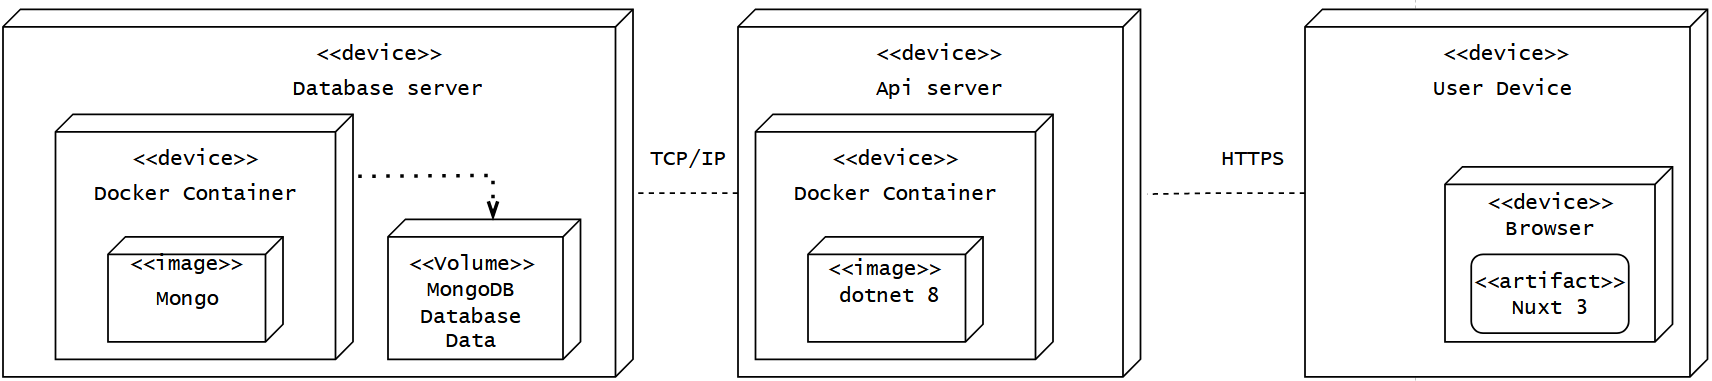
\includegraphics[scale=0.37]{DeploymentDiagram.png}
    \label{fig:DeploymentDiagram}
\end{graphic}

\todo[inline]{containariseren beter uitleggen en Frontend toevoegen aan het deployment diagram}
